\subsubsection{Pogon}
Deluje na principu vzvodov in krivulj. Imamo glavno krivuljno
vreteno, ki se vrti sinhronizirano s pogonom glavnega vretena
preko zobnikov, s katerimi preko tabele izbiramo čas cikla enega
kosa, saj se za en obrat krivuljnega vretena izvede en cikel.

Na spodnji Sliki \ref{pogon} je v pogledu od zgoraj prikazana shema
nekaterih delov enovretenske avtomatske stružnice Gauthier GM-127. Pod številko 21 in 18
so narisana ležajna mesta, skozi katera gre glavna krivuljna gred.
Pravokotno na njo so na raznih mestih vpete krivulje, ki preko sledilcev
in vzvodov premikajo razne dele stroja. Pod številko 19 je narisano
glavno vreteno, pod številko 31 pa nasprotna vretena, kamor se vpenjajo svedri.
\begin{figure}[H]
	\begin{center}
		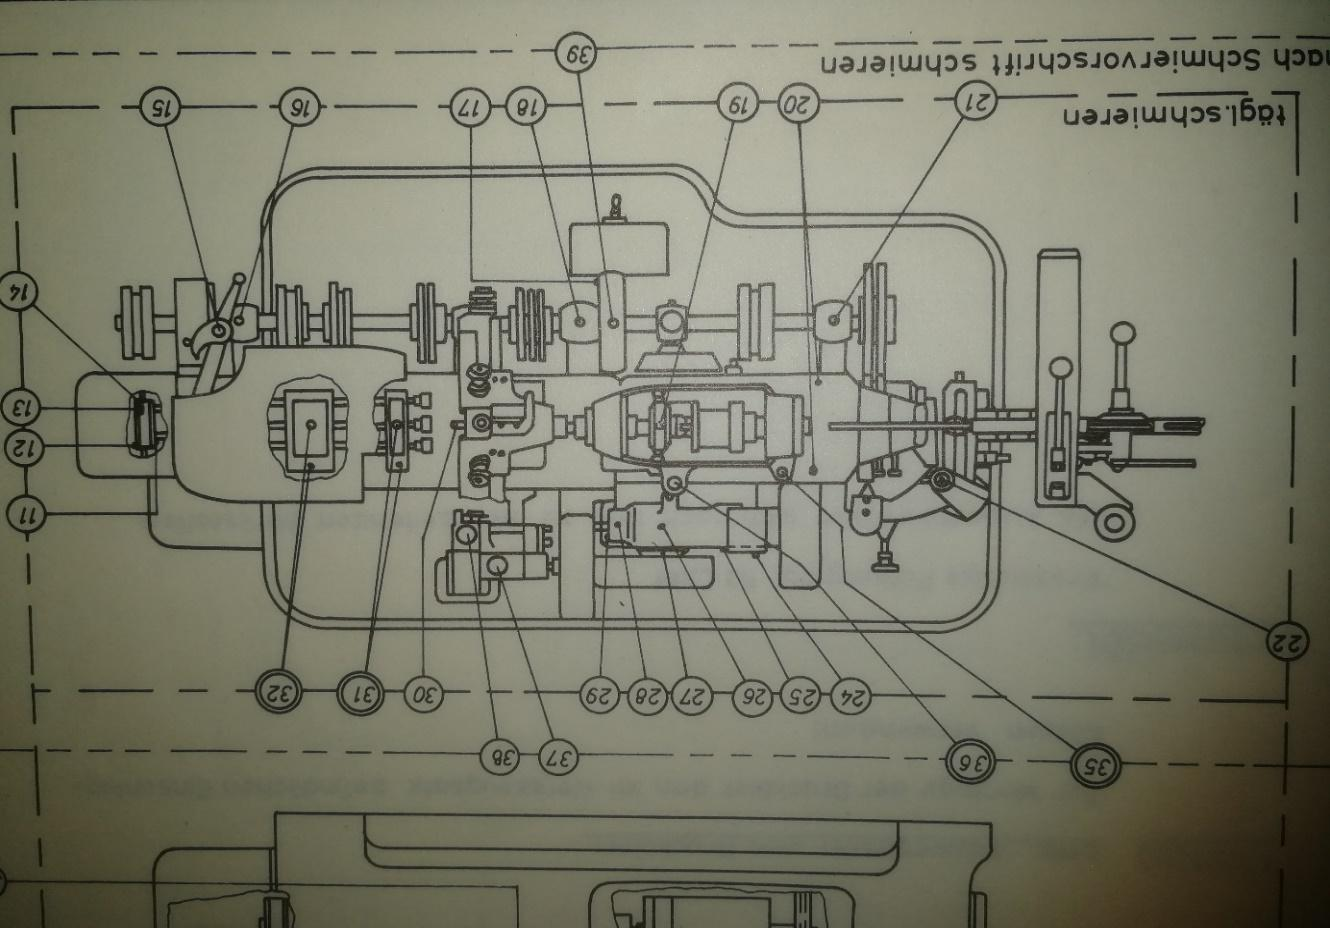
\includegraphics[width=\linewidth]{shema_avtomata.jpg}
		\caption{Shema delov enovretenske avtomatske stružnice
			\cite{gauthier}}
		\label{pogon}
	\end{center}
\end{figure}
Za pogon se največkrat uporablja običajen trofazni elektromotor,
ki preko menjalnika vrti glavno vreteno, krivuljno gred in ostala
pomožna vretena. Poznamo pa dve vrsti menjalnikov
\begin{itemize}
	\item Avtomatski -- s krivuljo lahko izbiramo med polno
	      hitrostjo, \( \frac{1}{2} \), \( \frac{1}{3} \), \( \frac{1}{4} \)
	      polne hitrosti ali pa zamenjamo
	      smer obratov (uporabno za vrezovanje navojev).

	\item Ročni -- hitrost se nastavlja ročno z izbiro zobnikov
	      v menjalniku in se med obratovanjem ne more spreminjati.
\end{itemize}

\subsubsection{Vpetje obdelovanca}
Avtomatske stružnice uporabljajo za vpetje izključno stročnice,
saj so najnatančnejši in najhitrejši način vpenjanja. Imajo pa nekaj slabosti,
in sicer se hitro zamažejo z ostružki, ti jih pa hitro uničijo,
njihov razpon vpetja je zelo majhen -- navadno največ okoli 1 mm. V stročnico z
izvrtino ø12 lahko vstavimo kos s premerom od ø11,5 do ø12,5,
zato je potrebno menjati stročnico skoraj vedno, kadar se stroj nastavlja.
Poznamo dva načina vpetja pri avtomatih:
\begin{itemize}
	\item Dolgostružno: Sistem dveh stročnic, ki se vrtijo z
	      enakimi obrati. Sprednja stročnica -- vodilna -- kosa ne vpne,
	      ampak ga vodi, da ne opleta in se lahko struženje izvaja čim
	      bližje vpetju. Zadnja stročnica pa surovec vpne in ga podaja
	      skozi vodilno stročnico.
	\item Kratkostružno: Sistem ene stročnice, ki vpne surovec
	      ter ga ne vodi skozi vodilno stročnico, tako da struženje
	      poteka dlje od vpetja, kar se pri obdelovancih manjših
	      premerov pozna v ekscentričnosti stružnih površin in tudi v obdelavi.
	      Večji kot je premer obdelovanca, dlje lahko gleda surovec iz stročnice.
	      Navadno se držimo pravila 3d, kar pomeni, da lahko obdelovanec visi
	      iz vpetja za največ tri-kratnik svojega premera.
\end{itemize}

Na spodnji Sliki \ref{tipi_vodilnih_pus} je na levi strani prikazana
shema dolgostružne konfiguracije, na desni pa kratkostružna konfiguracija
stročnic na avtomatski stružnici.

\begin{figure}
	\begin{center}
		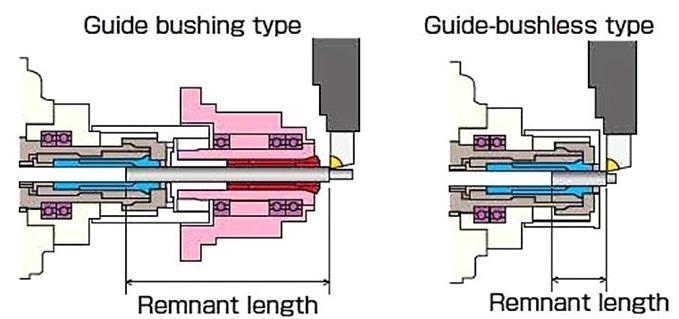
\includegraphics[width=\linewidth]{skuca_dolgo_struzenje.jpg}
		\caption{Shema postavitve pri dolgem struženju s stročnicami
			\cite{interna}}
		\label{tipi_vodilnih_pus}
	\end{center}
\end{figure}

Prednosti dolgostružnih avtomatov je daljša dolžina struženja
in boljše vpetje obdelovanca, zato je bolj primerna za daljše
kose manjših premerov. S primerno podporo se lahko obdeluje
tudi po celotni dolžini materiala.

Prednost kratkostružnih avtomatov je krajši ostanek palice,
saj sta vodilna puša in vpenjalna stročnica med seboj oddaljena, pri čemer vpenjalna stročnica ne more v celoti poriniti palice skozi vpenjalno
stročninco. Slabost pa je krajša dolžina struženja, saj je material
fiksno vpet in lahko pri manjših premerih, ki so dlje vpeti, pride
do zvijanja.

\subsubsection{Podajanje obdelovancev}
Za podajanje se uporabljajo podajalne naprave, ki podajajo
obdelovanec s hidravliko ali pa z utežmi. Hidravlična podajalna
naprava lahko večinoma sprejme več kot eno palico in jih tudi sama
zamenja ter vstavi v stroj. Možno je tudi nastavljati moč in dolžino
podajanja. Obstajajo tudi revolverske hidravlične podajalne naprave,
ki imajo ločene cevi, navadno 6, ki delujejo kot hidravlični cilinder
in porivajo palice proti stružnici.

Spodaj, na Sliki \ref{hidrobar_nalaganje} je prikazan postopek
avtomatskega nalaganja novega obdelovanca v kanal hidrobara.
Navadno imajo hidrobari zalogovnik za neko število palic, odvisno
od premera samega materiala. Ko hidrobar zazna, da v obdelovalnemu
kanalu ni več materiala, se obdelovalni kanal odpre in preko posebnega
mehanizma vanj pade samo ena palica. Ta se lahko nabije v posebne
stročnice, ki so nameščene na podajalni bat in tako omogočajo, da se
material pomika v stružnico ter se po koncu obdelave tudi izvleče ostanek.
Lahko pa se tudi uporabi brez stročnice na podajalnem batu, v tem primeru izgubimo sposobnost premikanja palice v obe smeri in moramo ostanek z
naslednjo vstavljeno palico izriniti skozi stročnice.
\begin{figure}[H]
	\begin{center}
		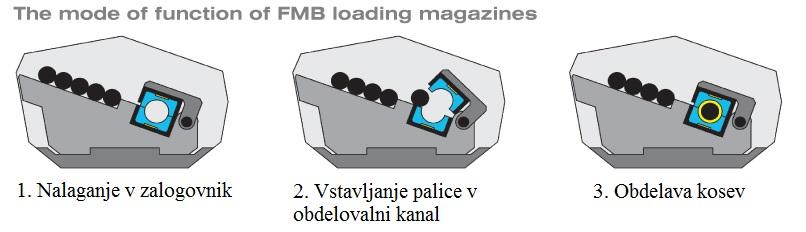
\includegraphics[width=15cm]{hidrobar_shema.jpg}
		\caption{Shema delovanja hidrobara
			\cite{interna}}
		\label{hidrobar_nalaganje}
	\end{center}
\end{figure}



Obstajajo tudi podajalci, ki za vstavljanje palice uporabljajo
utež. Ti so veliko cenejši in lažji za postavitev, izdelavo in nastavitev.
V njih lahko vstavimo samo eno palico materiala, pri čemer je potrebna ročna menjava
palice po koncu obdelave. Zaradi tega se največkrat uporabljajo za
krivuljne avtomate.

Na spodnji Sliki \ref{shema_rocnega_podajalca} je prikazana shema
delovanja ročnega podajalca palic. Pri menjavi iz stročnic na batu za podajanje
odstranimo ostanek palice, navadno dolg nekje do 20 cm. Nato previdno
vstavimo v stročnice novo palico in jo ročno porinemo do konca cevi.
Pri tem preko vrvi dvigujemo utež, ki mora biti ravno prav balansirana,
da nam omogoča enostavno vstavljanje kot tudi dovoljšno silo pri samodejnem
delovanju.

\begin{figure}[H]
	\begin{center}
		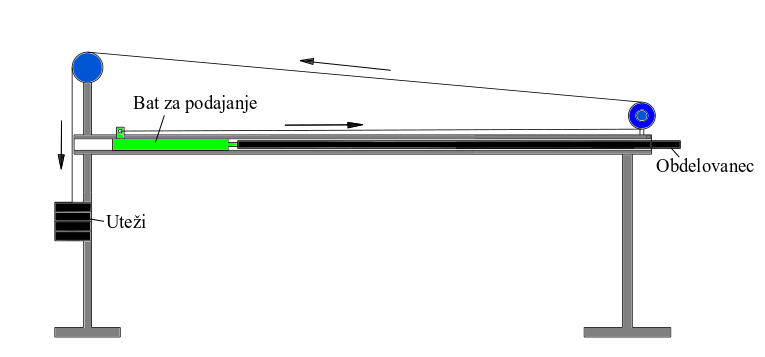
\includegraphics[width=15cm]{podajalec_utez.png}
		\caption{Ročni podajalec palic
			\cite{interna}}
		\label{shema_rocnega_podajalca}
	\end{center}
\end{figure}

\subsubsection{Krivuljna gred}
Je krmilni del vsakega krivuljnega avtomata. Vsebuje krivulje,
ki so največkrat iz kaljenega jekla, odpornega proti obrabi. Za en
obrat krivuljnega vretena se zaključi en cikel obdelovanja in je
izdelan eden izdelek (lahko tudi več, odvisno od nastavitve stroja).
Hitrost obračanja se lahko spreminja s prestavinimi razmerji
zobnikov, imamo pa tudi že vnaprej pripravljeno tabelo, po kateri
lahko izbiramo željeno hitrost in potrebne zobnike. Krivulje nato
preko sledilcev in vzvodov premikajo prečne suporte,
revolverske sani, vpenjajo in izpenjajo obdelovanec ...

\noindent Poznamo dve vrsti krivulj:
\begin{itemize}
	\item Navadne -- ploščate krivulje: uporabljamo jih za prečne pomike.
	\item Bobnaste krivulje: uporabljamo jih za vzdolžne pomike, navadno
	      sestavljene iz več segmentov.
\end{itemize}

Krivuljna gred se lahko vklopi ali izklopi s pomočjo ročne sklopke,
lahko pa se tudi ročno obrača preko te sklopke in se uporablja, kadar
se stroj nastavlja ali menja orodje. Sklopka ima vgrajen
zatič, ki se ob potencialnem strojelomu pretrga in ustavi vrtenje
krivuljne gredi, vendar se glavni motor ob tem ne izklopi.
Tukaj lahko pride do velikega trenja, če se orodje zaleti v
material, stročnico ali ostale rotirajoče dele, kar lahko
potencialno povzroči vžig mazalnega ali hladilnega olja.

Za izdelavo krivulj je potrebno veliko časa, saj
se nenatančnosti geometrije poznajo na končnem izdelku. Zato je
veliko krivulj standardiziranih in imajo vnaprej določen kot in
višino vzpona, zaradi česar se lahko stroj hitreje nastavi. Krivuljo po
meri se izdeluje samo, če je serija kosov dovolj velika in če ni
nikakršne druge možnosti. Največkrat se jih po meri izdeluje,
če potrebujemo neko obdelavo, ki je sestavljena iz več gibov,
kot npr. struženje kompleksnih kontur, širokih utorov, vrtanje
globokih lukenj ... Pri tem nam zelo prav pridejo računalniška
orodja, v katerih lahko krivuljo narišemo kot enostavno ravno
črto pod nekim vzponom in jo potem ovijemo okoli kroga ter dobimo
obliko krivulje, ki jo lahko uporabimo pri izdelavi.
